\documentclass[sigconf]{acmart}
\usepackage{xcolor}
\usepackage{graphicx}
% --- Added for the diagrams ---
\usepackage[edges]{forest}          % hierarchy tree (Fig. 1)
\usetikzlibrary{positioning,arrows.meta,fit}  % positioning diagram (Fig. 3)
% ------------------------------------------------
% Remove ACM-specific publication information
% if this is a course/project submission.
% ------------------------------------------------
\settopmatter{printacmref=false}
\setcopyright{none}
\acmConference{}{}{}
\acmBooktitle{}
\acmPrice{}
\acmDOI{}
\acmISBN{}
\renewcommand\footnotetextcopyrightpermission[1]{} % removes empty ACM footnote box

\begin{document}

% ------------------------------------------------
% TITLE
% ------------------------------------------------

\title{Recommendation Systems Background and Related Works}

% ------------------------------------------------
% AUTHORS
% ------------------------------------------------

\author{Thai Hung Vuong}
\affiliation{
    \institution{University of Victoria}
}
\email{thaihungvuong@uvic.ca}

\author{Brendan Wong}
\affiliation{
    \institution{University of Victoria}
}
\email{brendanwong@uvic.ca}

\author{Robert Legassicke}
\affiliation{
    \institution{University of Victoria}
}
\email{roblegs@uvic.ca}

\author{Yashwanthkrishna Nagharaj}
\affiliation{
    \institution{University of Victoria}
}
\email{yashwanthk@uvic.ca}

% ------------------------------------------------
% MAKE TITLE
% ------------------------------------------------

\maketitle

% ------------------------------------------------
% ABSTRACT
% ------------------------------------------------

\section*{Abstract}

This paper provides a concise overview of the concepts, approaches, and state of the art in academic major recommendation and student-program matching. In particular, we review existing recommendation systems, machine learning techniques, and approaches for matching students' skills and interests with suitable academic programs. We also examine how these approaches can be applied to MajorMatch, a system designed to support students to understand the connection between their latent proficiency and potential academic major. \href{https://github.com/yashwanth973/CSC503.git}
{\textcolor{blue}{\underline{https://github.com/yashwanth973/CSC503.git}}}.

\setcounter{section}{1}
\setcounter{subsection}{0}

\subsection{INTRODUCTION}
Students have varying skills, interests, and preferences, which makes selecting a suitable major challenging. Existing academic and career recommendation systems attempting to address these problems have been widely developed by using different approaches to match students with suitable educational or career pathways. These approaches vary in techniques and results. Some systems rely on predefined rules or direct matching between characteristics and program requirements, while others rely on identifying similarities between users and available programs. More data-driven approaches also use machine learning to learn and make predictions. Each approach provides different advantages and limitations in terms data requirements, flexibility, and accuracy. Major Match is a web-based system designed to recommend university majors based on student's skills. The application focuses on undergraduate majors at the University of Victoria (UVic). Rather than assuming that one approach is universally suitable, this project examines the existing solution space to determine how different recommendation approaches can be applied to academic major selection. This review compares these approaches, discusses their strengths and limitations, and establishes the position of MajorMatch within existing work.

\subsection{HISTORY}
% EDIT: author-name citations replaced with \cite; citations added for Parsons and the 1990s recommender systems.
The problem of matching individuals with suitable educational and career paths predates modern computing. Older recommendation systems relied on content-heavy media and used basic search filtering to assist users~\cite{rances}. In 1909, Frank Parsons proposed a systematic approach to vocational guidance based on understanding an individual's interests and abilities and comparing them with the requirements of different occupations~\cite{parsons}. As the number of educational and career options grew, computer-based systems provided new ways to organize this information and automate the matching process. During the 1990s, recommender systems introduced computational methods for providing personalized recommendations based on user preferences and similarities between users~\cite{resnick1994,resnick1997}. These ideas were later applied to education and career guidance, with modern systems increasingly using machine learning and data mining to identify patterns in student data. MajorMatch builds on this evolution by applying recommendation techniques to the problem of matching students' skills, interests, and preferences with potential university majors.

% ------------------------------------------------
% 1.3 HIERARCHY  (NEW SECTION + FIGURE 1)
% NOTE: this paragraph was drafted with AI -- rewrite it in your own words
% to comply with the course's "AI-Assisted Editing" policy.
% ------------------------------------------------
\subsection{HIERARCHY}
We categorize existing approaches by \emph{where the student--program mapping comes from} (Figure~\ref{fig:hierarchy}). \textbf{Knowledge-driven} approaches use a mapping fixed by people, either from vocational theory, such as Parsons' trait--factor matching~\cite{parsons}, or from expert scoring matrices behind questionnaires such as WorkBC~\cite{workbc} and the Major Match quiz~\cite{majormatch}. \textbf{Data-driven} approaches learn the mapping and are further divided by the data they learn from: \emph{content-based} methods learn from program or occupation text (TopProRec~\cite{hill}, O*NET interest profiles~\cite{javalagi}); \emph{student/outcome-based} methods learn from other users or successful students (collaborative filtering~\cite{resnick1994}, MyMajors~\cite{mymajors}); and \emph{hybrid} methods combine several learners (CoDeRS~\cite{rances}).

\begin{figure}[t]
\centering
\resizebox{\columnwidth}{!}{%
\begin{forest}
  for tree={
    font=\footnotesize, draw, rounded corners=2pt, align=center,
    grow'=0, anchor=west, child anchor=west, parent anchor=east,
    s sep=3pt, l sep=10pt, fork sep=5pt,
    forked edges, edge={rounded corners=1pt},
  },
  where level=0{fill=gray!20, font=\footnotesize\bfseries}{},
  where level=1{fill=gray!8, font=\footnotesize\bfseries}{},
  [Student--Program\\Recommendation
    [Knowledge-driven\\(pre-defined)
      [Trait--factor theory\\{Parsons~\cite{parsons}}]
      [Expert scoring matrices\\{WorkBC~\cite{workbc}, Major Match~\cite{majormatch}}]
    ]
    [Data-driven\\(learned)
      [Content-based (program text)\\{TopProRec~\cite{hill}, O*NET~\cite{javalagi}}, line width=0.9pt, fill=blue!8]
      [Student/outcome-based\\{GroupLens~\cite{resnick1994}, MyMajors~\cite{mymajors}}]
      [Hybrid / ensemble\\{CoDeRS~\cite{rances}}]
    ]
  ]
\end{forest}}
\caption{Taxonomy of student--program recommendation approaches. The shaded box marks MajorMatch's starting point.}
\label{fig:hierarchy}
\end{figure}

% ------------------------------------------------
% 1.4 COMPARATIVE ANALYSIS
% (removed \setcounter{section}{2} so numbering continues 1.3, 1.4, 1.5 as in the manual)
% ------------------------------------------------
\subsection{COMPARATIVE ANALYSIS}
CoDeRS~\cite{rances} is a data driven web based recommendation system designed to give students recommended computing degree programs based on academic data, personality traits, interests, hobbies, and career aspirations. It collects data by integrating user profiles, then looks at users' hobbies, skills, etc. The software utilises approaches like Multinomial Naive Bayes for text classification of students profiles, content-based filtering (CBF) for analyzing academic and text data. Additionally, the application used The Big Five inventory and cosine similarity to match personalities. CoDeRS would recommend a program to a user if it was recommended by at least two algorithms from the aforementioned approaches.
This multi-factor approach lets CoDeRS consider a wide range of data, increasing accuracy of recommendations. The model works without the need of a very large dataset, which will fit our needs for a project. The author does note that this approach is dependent on the profiles they have on hand and are limited to profiles they were able to gather.

Questionnaires use different strategies to determine the result of a student's prompts in the questionnaires. Some examples include:

% EDIT: O*NET description corrected -- its interest profiles are generated by ML
% from occupation text, not refined from surveys of workers (see [javalagi]).
\begin{itemize}
    \item \textbf{WorkBC Quizzes}~\cite{workbc} -- use a pre-defined rigid matrix to determine the outcomes of student responses.
    \item \textbf{O*Net Interest Profiler}~\cite{onet} -- scores interests with a fixed questionnaire, but the occupational profiles it matches against are generated by machine-learning models trained on occupation text and expert ratings, and are updated with each database release~\cite{javalagi}. A model that improves over time is the goal we are trying to create in our own project.
\end{itemize}
Most of the other questionnaires that exist follow one of these two formats: Pre-defined model, or adaptive model.

Systems that match high school students to programs are limited, each uses a different approaches and modeling system:
% EDIT: MyMajors description corrected -- the source only says it is built on data about student success, not 4th-year students specifically.
\begin{itemize}
    \item \textbf{Major Match (not our project)}~\cite{majormatch} -- This questionnaire includes more gimmicky questions, including picking your favourite option from a set of options, and uses a pre-defined matrix. Given its game-like ``quicktime'' questioning, it is more of a fun game than an actual serious questionnaire.
    \item \textbf{MyMajors}~\cite{mymajors} -- Uses a questionnaire covering academic achievement, interests, temperament and values, and matches students using data on what it takes to succeed in different fields of study. This is closer to the approach we are trying to pursue in our project.
\end{itemize}
Overall, these tools range from fixed matrices, either game-like (Major Match) or expert-built (WorkBC), to models that are updated with data (O*NET, MyMajors). Figure~\ref{fig:venn-table} summarizes these comparisons.

\begin{figure}[t]
    \centering
    \begin{minipage}{0.48\columnwidth}
        \centering
        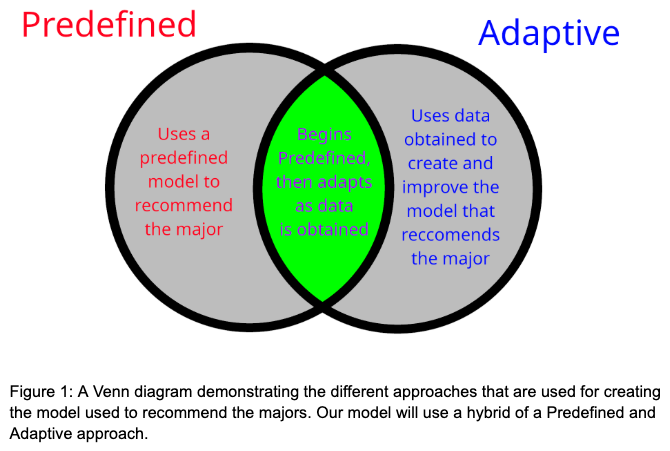
\includegraphics[width=\linewidth]{VENDIAGRAM.png}
        \\{\small (a) Venn diagram}
    \end{minipage}
    \hfill
    \begin{minipage}{0.48\columnwidth}
        \centering
        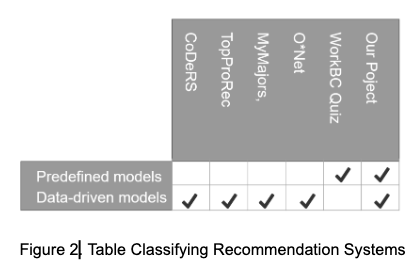
\includegraphics[width=\linewidth]{TABLE.png}
        \\{\small (b) Comparison table}
    \end{minipage}
    \caption{Overlap (a) and feature comparison (b) of the reviewed approaches.}
    \label{fig:venn-table}
\end{figure}

% ------------------------------------------------
% 1.5 POSITION YOUR PROJECT  (+ FIGURE 3)
% NOTE: much of this section is AI-written text -- rewrite it in your own words
% and condense it, per the course's "AI-Assisted Editing" policy.
% ------------------------------------------------
\subsection{PROJECT POSITIONING}
As Figure~\ref{fig:hierarchy} shows, existing approaches are either knowledge-driven, which are transparent and need no data but cannot improve, or data-driven, which capture complex relationships and improve over time but need representative data that a new, institution-specific system does not have. MajorMatch is an application-based project: rather than proposing a new algorithm, it adapts established techniques to recommending UVic undergraduate majors from a student's latent proficiencies (Figure~\ref{fig:position}). It \textbf{builds on} CoDeRS~\cite{rances}, adopting similarity-based matching between a student's proficiency profile and each major's profile, which works without a large dataset. It \textbf{adapts} TopProRec~\cite{hill}, building major profiles from UVic course and program descriptions so the system works before any student data exists. It is \textbf{inspired by} O*NET~\cite{javalagi} and MyMajors~\cite{mymajors}, which keep their models up to date with new data; student feedback and outcomes could likewise recalibrate MajorMatch over time. Fixed-matrix tools such as WorkBC~\cite{workbc} and the Major Match quiz~\cite{majormatch} serve as \textbf{baselines}. No existing tool covers UVic's programs or matches on proficiency, so the contribution is applying proven techniques to this new domain and investigating which combination of rule-based, similarity-based and adaptive methods works best when data is limited at the start.

\begin{figure}[t]
\centering
\resizebox{\columnwidth}{!}{%
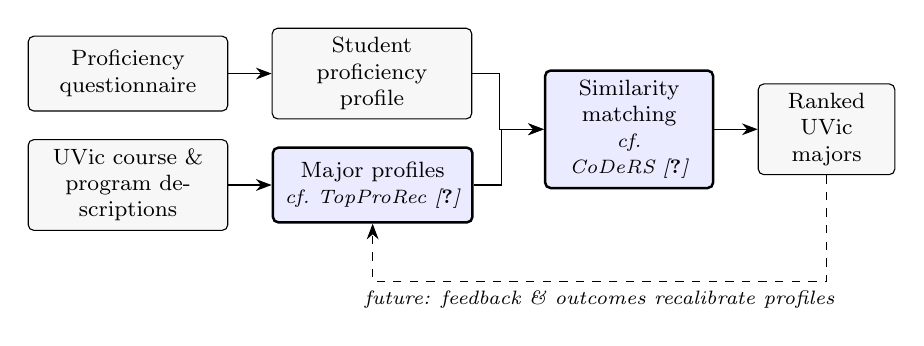
\begin{tikzpicture}[
  font=\footnotesize,
  box/.style={draw, rounded corners=2pt, align=center, minimum height=0.95cm, text width=2.3cm, fill=gray!6},
  key/.style={box, fill=blue!8, line width=0.9pt},
  >={Stealth[length=2mm]}, node distance=0.35cm and 0.55cm]
  \node[box] (q)  {Proficiency\\questionnaire};
  \node[box, right=of q] (sp) {Student\\proficiency profile};
  \node[box, below=of q] (cd) {UVic course \&\\program descriptions};
  \node[key, right=of cd] (mp) {Major profiles\\{\scriptsize\itshape cf.\ TopProRec~\cite{hill}}};
  \node[key, right=0.9cm of $(sp.east)!0.5!(mp.east)$, text width=1.9cm] (sim) {Similarity\\matching\\{\scriptsize\itshape cf.\ CoDeRS~\cite{rances}}};
  \node[box, right=of sim, text width=1.5cm] (out) {Ranked\\UVic majors};
  \draw[->] (q) -- (sp);
  \draw[->] (cd) -- (mp);
  \draw[->] (sp.east) -- ++(0.35,0) |- (sim.west);
  \draw[->] (mp.east) -- ++(0.35,0) |- (sim.west);
  \draw[->] (sim) -- (out);
  \draw[->, dashed] (out.south) |- ++(0,-1.35) -| (mp.south)
    node[pos=0.25, below, font=\scriptsize\itshape]{future: feedback \& outcomes recalibrate profiles};
\end{tikzpicture}}
\caption{How MajorMatch combines the reviewed approaches. Shaded boxes are the parts drawn from existing work; the dashed loop is the planned adaptive refinement.}
\label{fig:position}
\end{figure}

% ------------------------------------------------
% REFERENCES
% (citation keys renamed: keys with spaces such as {Province of BC} break \cite)
% ------------------------------------------------

\begin{thebibliography}{10}

\bibitem{hill}
A. Hill, K. Goo, and P. Agarwal, ``Recommending the right academic programs: An interest mining approach using BERTopic,'' \textit{Data Mining and Knowledge Discovery}, vol. 39, no. 3, Mar. 2025, doi: 10.1007/s10618-024-01087-y.

\bibitem{rances}
C. A. Rances, R. A. Sipe, S. Baris, A. Lopez, A. D. Rosaldo, R. Bringula, and S. U. Ulfa, ``CoDeRS: A computing degree program recommender system using machine learning algorithms,'' \textit{Frontiers in Artificial Intelligence}, vol. 9, Art. no. 1874202, Jul. 2026, doi: 10.3389/frai.2026.1874202.

\bibitem{parsons}
F. Parsons, \textit{Choosing a Vocation}. Boston, MA, USA: Houghton Mifflin, 1909.

\bibitem{workbc}
Province of British Columbia, ``Career Discovery Quizzes,'' WorkBC, 2026. \url{https://careerdiscoveryquizzes.workbc.ca/}

\bibitem{onet}
National Center for O*NET Development, ``O*NET Interest Profiler,'' U.S. Department of Labor, Employment and Training Administration. \url{https://onetinterestprofiler.org/}

\bibitem{majormatch}
Major Match, ``Major Match: Find your university major.'' \url{https://majormatch.io/}

\bibitem{mymajors}
MyMajors, ``College Major Quiz.'' \url{https://www.mymajors.com/college-major-quiz/}

\bibitem{javalagi}
A. A. Javalagi and J. A. Dahlke, ``Updates to occupational interest profiles and high-point codes for the O*NET program using the O*NET 30.0 database,'' National Center for O*NET Development, Raleigh, NC, USA, Tech. Memo. 2025-143, Jan. 2026.

\bibitem{resnick1994}
P. Resnick, N. Iacovou, M. Suchak, P. Bergstrom, and J. Riedl, ``GroupLens: An open architecture for collaborative filtering of netnews,'' in \textit{Proc. ACM Conf. Computer Supported Cooperative Work (CSCW '94)}, Chapel Hill, NC, USA, 1994, pp. 175--186, doi: 10.1145/192844.192905.

\bibitem{resnick1997}
P. Resnick and H. R. Varian, ``Recommender systems,'' \textit{Communications of the ACM}, vol. 40, no. 3, pp. 56--58, Mar. 1997, doi: 10.1145/245108.245121.

\end{thebibliography}

\end{document}